% catalogue: title = Nodes with shapes, colors and math content
% catalogue: min-coverage = 1.00
\documentclass[border=10pt]{standalone}
\PassOptionsToPackage{dvipsnames,svgnames,x11names}{xcolor}
\usepackage{tikz}
\usepackage{pgfplots}
\pgfplotsset{compat=newest}
\usepgfplotslibrary{groupplots}
\usetikzlibrary{arrows.meta,shapes.geometric}
\begin{document}
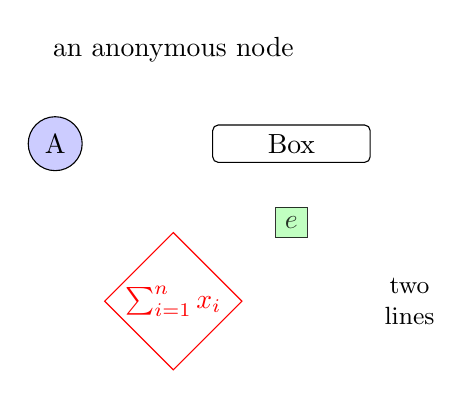
\begin{tikzpicture}
    \node[draw, circle, fill=blue!20] (a) at (0, 0) {A};
    \node[draw, rectangle, rounded corners=2pt, minimum width=2cm] (b) at (3, 0) {Box};
    \node[shape=diamond, draw=red, text=red, inner sep=1pt] (c) at (1.5, -2) {$\sum_{i=1}^n x_i$};
    \node at (1.5, 1.2) {an anonymous node};
    \node[align=center, font=\small] (d) at (4.5, -2) {two\\lines};
    \node[draw, fill=green!30, opacity=0.8] (e) at ({1+2}, {-1}) {$e$};
\end{tikzpicture}
\end{document}
